%
% حق نشر 1390-1402 دانش پژوهان ققنوس
% حقوق این اثر محفوظ است.
% 
% استفاده مجدد از متن و یا نتایج این اثر در هر شکل غیر قانونی است مگر اینکه متن حق
% نشر بالا در ابتدای تمامی مستندهای و یا برنامه‌های به دست آمده از این اثر
% بازنویسی شود. این کار باید برای تمامی مستندها، متنهای تبلیغاتی برنامه‌های
% کاربردی و سایر مواردی که از این اثر به دست می‌آید مندرج شده و در قسمت تقدیر از
% صاحب این اثر نام برده شود.
% 
% نام گروه دانش پژوهان ققنوس ممکن است در محصولات دست آمده شده از این اثر درج
% نشود که در این حالت با مطالبی که در بالا اورده شده در تضاد نیست. برای اطلاع
% بیشتر در مورد حق نشر آدرس زیر مراجعه کنید:
% 
% http://dpq.co.ir/licence
%
\part{نصب و استفاده}

در این بخش نحوه‌ی نصب و استفاده از ابزار \lr{Doxygen} توضیح داده می‌شود.
\lr{Doxygen} به خودی خود از طریق خط فرمان
قابل استفاده است. به عبارتی یک نرم‌افزار گرافیکی نیست. اما ابزاری برای استفاده
از این برنامه به صورت گرافیکی وجود دارد.
این ابزار \lr{Doxywizard} است. \lr{Doxywizard} یک واسط گرافیکی است که امکان
استفاده از \lr{Doxygen} را به صورت گرافیکی فراهم می کند. در این بخش علاوه بر
\lr{Doxygen}، نحوه‌ی نصب و استفاده از \lr{Doxywizard} نیز توضیح داده می‌شود.
  
ابزارهای تولید مستند \lr{Doxygen} و \lr{Doxywizard}، هم برای سیستم عامل ویندوز
و هم برای سیستم عامل‌های لینوکس وجود دارند.
درفصل نصب، نحوه‌ی نصب این ابزار بر روی هر دو سیستم عامل شرح داده شده است.
علاوه بر آن، از آنجا که سیستم عامل لینوکسی \lr{OpenSUSE} مدیریت خاص و البته
بسیار ساده و کاربرپسندی برای نصب برنامه‌ها دارد، نحوه‌ی نصب \lr{Doxygen} و
\lr{Doxywizard} بر روی این سیستم عامل نیز به طور جداگانه توضیح داده شده است.

در فصل استفاده، نحوه استفاده از \lr{Doxygen} هم از طریق خط فرمان و هم به صورت
گرافیکی (با استفاده از ابزار \lr{Doxywizard}) بیان شده است.



\chapter{نصب}
% در این فصل نشان داده می‌شود که چگونه باید این نرم‌افزار را نصب کرد، و برای
% تولید مستند از آن استفاده کرد.\cite{surhone2010doxygen}
 
برای نصب \lr{Doxygen} و \lr{Doxywizard} ابتدا باید آن‌ها را دریافت کنید. این
برنامه‌ها کاملا رایگان هستند.
در واقع \lr{Doxygen} یک نرم‌افزار متن باز\LTRfootnote{Open Source} است. متن
این برنامه و همچنین پرونده‌ی قابل اجرای آن را می‌توان از آدرس
\url{http://www.doxygen.org/download.html} 
دریافت کرد. برای نصب این برنامه می‌توانید متن آن را دریافت کنید و سپس آن را
روی سیستم خود ترجمه (کامپایل) کنید و از آن استفاده کنید. روش دیگر هم این است
که از برنامه‌های ترجمه شده و قابل اجرایی که روی آدرس ذکر شده قرار دارد
استفاده کنید. در این کتاب فقط روش دوم را شرح می‌دهیم، چون روش عمومی‌تری است.

% در این قسمت نحوه‌ی نصب بر روی سیستم عامل اوپن سوزی شرح داده می شود. به دلیل اینکه در اوپن سوزی
% روشی ساده با گرافیکی کاربرپسند برای نصب برنامه ها وجود دارد، نصب روی این سیستم عامل را به طور جداگانه
% علاوه بر سیستم عامل‌های لینوکسی آورده‌ایم.
% محمد هادی منصوری ۹۰/۳/۳
\section{\lr{OpenSUSE}}

اگرچه دستورالعمل مربوط به نصب \lr{Doxygen} روی سیستم عامل‌های لینوکسی برای سیستم
عامل \lr{OpenSUSE} هم قابل استفاده است، اما سیستم عامل \lr{OpenSUSE} روشی
گرافیکی ساده و کاربرپسندی برای نصب برنامه‌ها دارد.
در این سیستم عامل مدیریت گرافیکی \lr{YaST} امکانات مناسبی برای مدیریت قسمت‌های
مختلف سیستم فراهم آورده است.
از جمله‌ی این امکانات مدیریت مخزن‌ها\footnote{\lr{Repository}}و مدیریت
نرم‌افزارها\footnote{\lr{Software Management}} است.

برای نصب \lr{Doxygen}، ابتدا باید به اینترنت وصل باشید. سپس از طریق منوی شروع در
\lr{OpenSUSE} که با علامت 
\includegraphics[width=0.5cm]{image/opensuse} نشان
داده می‌شودبرنامه‌ی \lr{YaST} را اجرا کنید. سپس قسمت \lr{Software Management} را
انتخاب کنید. پس از اینکه ابزار مدیریت نرم‌افزارها باز شد، در قسمت جستجو، کلمه‌ی
\lr{doxy} را جستجو کنید. در فهرستی که از نتیجه‌ی جستجو نشان داده می‌شود
برنامه‌های \lr{doxygen} و \lr{doxywizard} را به حالت انتخاب در آورید، و سپس
دکمه‌ی تایید را بزنید تا سیستم شروع به نصب برنامه‌ها کند. هر کدام از این
برنامه‌ها که قبلا روی سیستم شما نصب شده باشند به حالت انتخاب شده هستند و نیازی
به نصب آن ندارید. البته ممکن است که بخواهید آن برنامه را به‌روز کنید. تصویر
\ref{image/install/OpenSUSE/setup} را مشاهده کنید.

\begin{figure}
 \centering
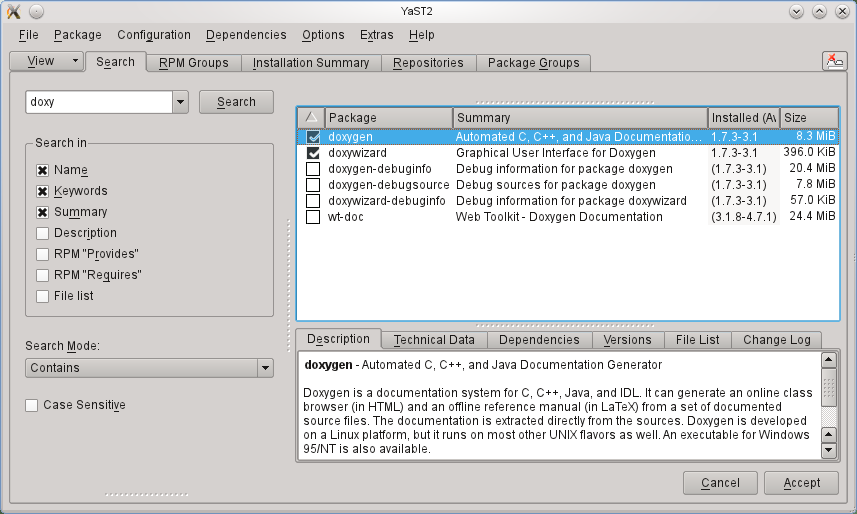
\includegraphics[width=0.75\textwidth]{image/install/OpenSUSE/setup}
\caption[پنجره‌ی نصب برنامه‌ها در سیستم عامل \lr{OpenSUSE}.]{
پنجره‌ی نصب برنامه‌ها در سیستم عامل \lr{OpenSUSE}. پس از جستجوی نام ابزار مورد
نظر خود، آن‌ها را انتخاب کرده و سپس شروع به نصب کنید.
}
\label{image/install/OpenSUSE/setup}
\end{figure}

در صورتی که \lr{doxygen} یا \lr{doxywizard} در نتایج جستجو مشاهده نشد، احتمالا
مخزن مربوط به این نرم‌افزارها در فهرست مخزن‌های سیستم شما وجود ندارد و باید آن
را اضافه کنید. برای این کار ابتدا آدرس یک مخزن که این ابراز را دارد پیدا کنید
سپس در \lr{YaST} به قسمت \lr{Software Repositories} رفته و این آدرس را به فهرست
مخزن‌های سیستم اضافه کنید. پس از آن دوباره نام ابزارها را جستجو کنید و آن‌ها را
نصب کنید.


% در این قسمت نحوه‌ی نصب، روی سیستم عامل های لینوکسی شرح داده می شود.
% محمد هادی منصوری ۹۰/۳/۲
%
% حق نشر 1390-1402 دانش پژوهان ققنوس
% حقوق این اثر محفوظ است.
% 
% استفاده مجدد از متن و یا نتایج این اثر در هر شکل غیر قانونی است مگر اینکه متن حق
% نشر بالا در ابتدای تمامی مستندهای و یا برنامه‌های به دست آمده از این اثر
% بازنویسی شود. این کار باید برای تمامی مستندها، متنهای تبلیغاتی برنامه‌های
% کاربردی و سایر مواردی که از این اثر به دست می‌آید مندرج شده و در قسمت تقدیر از
% صاحب این اثر نام برده شود.
% 
% نام گروه دانش پژوهان ققنوس ممکن است در محصولات دست آمده شده از این اثر درج
% نشود که در این حالت با مطالبی که در بالا اورده شده در تضاد نیست. برای اطلاع
% بیشتر در مورد حق نشر آدرس زیر مراجعه کنید:
% 
% http://dpq.co.ir/licence
%
\section{لینوکس}
\label{install/linux}

\begin{sloppypar}
برای نصب \lr{Doxygen} روی سیستم عامل‌های لینوکسی نیاز به توزیع دودویی مناسب برای سیستم عامل خود دارید. از آدرس 
\url{http://www.doxygen.org/download.html}
 می‌توانید توزیع مناسب را دریافت کنید. پس از دریافت توزیع مناسب، با دستورات زیر می‌توان \lr{Doxygen} را نصب کرد. 
معمولا بین پرونده‌های دریافت شده، پرونده‌ای به نام \lr{configure} وجود دارد. این پرونده حاوی دستورات خط فرمان (دستورات شل) برای 
پیکربندی اولیه است. دستورات زیر پیکربندی اولیه را انجام داده و برنامه را نصب می‌کند.
\end{sloppypar}
\begin{latin}
\lstset{language=C++}  
\begin{lstlisting}[frame=single] 
./configure
make install
\end{lstlisting}
\end{latin}
%\begin{flushleft}
%\lr{./configure} \\
%\lr{make install}
%\end{flushleft}
برای نصب مستندات و مثال‌ها دستور زیر را اجرا کنید.
\begin{latin}
\lstset{language=C++}  
\begin{lstlisting}[frame=single] 
make install_docs
\end{lstlisting}
\end{latin}
%\begin{flushleft}
%\lr{make install\_docs}
%\end{flushleft}
پرونده‌های اجرایی در مسیر 
\lr{<prefix>/bin}
 و مستندات و مثال‌ها در مسیر 
\lr{<docdir>/doxygen}
  نصب می‌شوند.

\begin{sloppypar}
به صورت پیش‌فرض 
\lr{<prefix>}
 به آدرس 
\lr{usr/local}
 اشاره دارد، اما می‌توان آن را با تغییر پارامتر 
\lr{--prefix}
 در پرونده‌ی \lr{configure} تغییر داد. 
\lr{<docdir>}
 نیز به صورت پیش‌فرض به آدرس 
\lr{<prefix>/share/doc/packages}
 اشاره دارد که این آدرس را نیز می‌توان با تغییر پارامتر 
\lr{--doxdir}
 در پرونده‌ی \lr{configure} عوض کرد.
\end{sloppypar}

در صورتی که از بسته‌های \lr{RPM} یا \lr{DEP} استفاده می‌کنید، همان روند استاندارد 
نصب را دنبال کنید که برای این بسته‌ها مورد نیاز است.


% در این قسمت نحوه‌ی نصب DoxyGen روی سیستم عامل ویندوز توضیح داده شده است.
% محمد هادی منصوری. ۹۰/۳/۱
%
% حق نشر 1390-1402 دانش پژوهان ققنوس
% حقوق این اثر محفوظ است.
% 
% استفاده مجدد از متن و یا نتایج این اثر در هر شکل غیر قانونی است مگر اینکه متن حق
% نشر بالا در ابتدای تمامی مستندهای و یا برنامه‌های به دست آمده از این اثر
% بازنویسی شود. این کار باید برای تمامی مستندها، متنهای تبلیغاتی برنامه‌های
% کاربردی و سایر مواردی که از این اثر به دست می‌آید مندرج شده و در قسمت تقدیر از
% صاحب این اثر نام برده شود.
% 
% نام گروه دانش پژوهان ققنوس ممکن است در محصولات دست آمده شده از این اثر درج
% نشود که در این حالت با مطالبی که در بالا اورده شده در تضاد نیست. برای اطلاع
% بیشتر در مورد حق نشر آدرس زیر مراجعه کنید:
% 
% http://dpq.co.ir/licence
%
\section{ویندوز}

در آدرس
\url{http://www.doxygen.org/download.html} 
یک برنامه‌ی اجرایی برای نصب نسخه‌ی ویندوزی وجود دارد. این برنامه به صورت یک
مجموعه کامل قابل نصب است و نصب آن بسیار ساده است.
کافی است پنجره‌های محاوره‌ای را دنبال کنید.



در هنگام نصب در یکی از مراحل از کاربر خواسته می‌شود موارد لازم برای نصب را تعیین کند. 
تصویر \ref{پنجره_نصب_روی_ویندوز} را ببینید. در این مرحله 
فهرستی از ابزارهایی که نصب می‌شودقرار داده شده است. 
همانگونه که در تصویر \ref{پنجره_نصب_روی_ویندوز} دیده می‌شود یکی از ابزارها، \lr{Doxywizard} است. 
به این ترتیب می‌توان در نسخه‌ی ویندوزی، هر دو ابزار \lr{Doxygen} و \lr{Doxywizard} را نصب کرد.

\begin{figure}
\centering
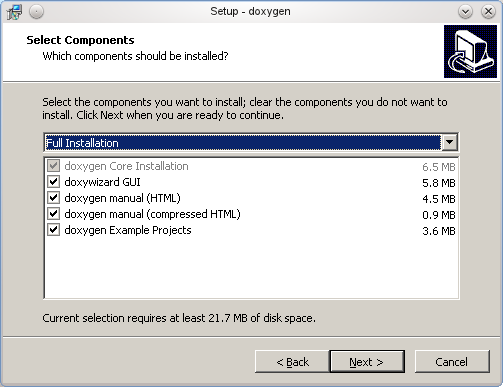
\includegraphics[width=0.75\textwidth]{image/windows_setup}
\caption[
پنجره‌ی محاوره‌ای نصب
{\lr{Doxygen}}
 روی ویندوز
]{
پنجره‌ی محاوره‌ای نصب
{\lr{Doxygen}}
 روی ویندوز. در این پنجره فهرستی از مواردی که باید نصب شود قرار دارد.
}
\label{پنجره_نصب_روی_ویندوز}
\end{figure}

توصیه می شود که بعد از نصب،
\lr{GraphViz} 
(نسخه‌ی ۲/۸ یا جدیدتر) را هم دریافت کرده و نصب کنید.
\lr{Doxygen}
 می تواند از ابزار
\lr{dot}
 مربوط به بسته‌ی
\lr{GraphViz}
، برای تولید بهتر دیاگرام ها استفاده کند.
% تنظیم \lr{HAVE\_DOT} در پرونده‌ی پیکربندی را مشاهده کنید.

اگر می‌خواهید پرونده‌های فشرده‌ی \lr{HTML} تولید کنید، نیاز به 
\lr{Microsoft HTML help} 
دارید. این ابزار را می‌توانید از آدرس 
\url{http://msdn.microsoft.com/en-us/library/ms670169}
 دریافت کنید.
%(تنظیم \lr{GENERATE\_HTMLHELP} را در پرونده‌ی پیکربندی مشاهده کنید)،

اگر می‌خواهید پرونده‌های فشرده‌ی \lr{Qt} را تولید کنید، نیاز به \lr{qhelpgenerator} دارید که قسمتی از \lr{Qt} 
 است. \lr{Qt} را می‌توانید از آدرس 
\url{http://qt.nokia.com/downloads/}
دریافت کنید.

به منظور تولید خروجی \lr{PDF}، یا استفاده از فرمول‌های خاص، احتیاج به نصب
\lr{LaTeX} و \lr{Ghostscript} دارید.
برای \lr{LaTex} چند توزیع وجود دارد. از جمله موارد معروف که باید با \lr{doxygen}
کار کنند \lr{MikTex} و \lr{XemTex} است\footnote{متاسفانه تولید مستند در قالب
\lr{LaTeX} با استفاده از \lr{Doxygen} برای مستندات به زبان فارسی با مشکلاتی
روبروست}.
\lr{Ghostscript} 
 را می‌توان از آدرس
\url{http://sourceforge.net/projects/ghostscript/} 
 دریافت کرد.

پس از نصب \lr{LaTex} و \lr{Ghostscript} باید مطمئن شوید که ابزارهای
\lr{latex.exe}، \lr{pdflatex.exe} و \lr{gswin32c.exe} در مسیر جستجوی دستورات خط
فرمان قرار دارند. در صورتی که از این موضوع مطمئن نیستید دستورالعمل زیر را دنبال
کنید و دستورات را در خط فرمان اجرا کنید تا ببینید به درستی کار می‌کنند یا نه.

از صفحه‌ی اصلی ویندوز روی \lr{My Computer} کلیک راست کرده و گزینه‌ی
\lr{Properties} را انتخاب کنید.
 در پنجره‌ای که ظاهر می‌شود زبانه‌ی \lr{Advanced} را انتخاب کنید. سپس دکمه‌ی
 \lr{Environment Variables} را کلیک کنید.
 در پنجره‌ای که ظاهر می‌شود متغیر \lr{Path} را انتخاب کرده و دکمه‌ی \lr{Edit} را
 کلیک کنید.
 سپس مسیرهای مربوط به ابزارهای گفته شده را در صورتی که وجود نداشت، در این قسمت
 اضافه کنید.
 مسیرهای مختلف با استفاده از علامت نقطه ویرگول از هم جدا می‌شوند. مثلا
\lr{C:\textbackslash Program Files;C:\textbackslash Winnt;C:\textbackslash
Winnt\textbackslash System32}.

پس از انجام کارهای گفته شده نرم‌افزار \lr{Doxygen} نصب شده و آماده استفاده است.



\chapter{نحوه استفاده}

%در این قسمت نحوه استفاده از doxygen و doxywizard آورده شده است. این بخش شامل دو زیر بخش خواهد بود
%یکی نحوه استفاده از doxygen به صورت خط فرمان و دیگری استفاده از doxygen به صورت گرافیکی که همان
%استفاده از doxywizard است.
%محمد هادی منصوری ۹۰/۳/۲۰
%\section {
%%نحوه‌ی استفاده از {\lr{Doxygen}} و {\{Doxywizard}}
%نحوه‌ی استفاده از Doxygen و Doxywizard
%}
در این قسمت  نحوه‌ی استفاده از \lr{Doxygen} و \lr{Doxywizard} توضیح داده شده است. 
برنامه‌ی اجرایی \lr{Doxygen} در واقع ابزار اصلی برای تولید مستند است. این برنامه پرونده‌های منبع\footnote{\lr{Source Files}} را تجزیه\footnote{\lr{Parse}}
 کرده و مستند مورد نظر را از پرونده‌های منبع تولید می‌کند. لازم به ذکر است که مستندات در پرونده‌های منبع باید 
به شکلی خاص نوشته شود، که نحوه‌ی نوشتن مستندات در پرونده‌های منبع در فصل‌های آتی توضیح داده شده است.

\lr{Doxygen} 
از یک پرونده‌ی پیکربندی\footnote{\lr{Configuration File}}
 برای تولید مستند استفاده می کند. در این پرونده‌ی پیکربندی، تنظیمات مربوط به نحوه‌ی تولید مستند، 
نوع پرونده‌های ورودی و خروجی، ظاهر مستند تولیدی و سایر تنظیمات قرار داده می‌شود. با ویرایش پرونده‌ی پیکربندی می‌توانیم تنظیمات 
دلخواه خود را برای \lr{Doxygen} تعیین کنیم.

\lr{Doxygen} 
اساسا یک ابزار کاربردی بر مبنای خط فرمان\footnote{\lr{Command Line}} 
است. بنابراین برای اجرا و استفاده از آن باید از طریق خط فرمان دستورات لازم را بدهیم. اما برخی ابزارهای گرافیکی وجود دارند 
که با استفاده از آن‌ها می‌توانیم \lr{Doxygen} را به صورت گرافیکی مورد استفاده قرار دهیم و نیازی به وارد کردن دستورات از طریق 
خط فرمان نیست. \lr{Doxywizard} یکی از این برنامه‌های گرافیکی است. با استفاده از \lr{Doxywizard} می‌توان یک پرونده‌ی پیکربندی 
ایجاد کرد یا یک پرونده‌ی پیکربندی را ویرایش کرد. همچنین با استفاده از این برنامه می‌توان \lr{Doxygen} را 
بدون نیاز به دستورات خط فرمان اجرا کرد. در تصویر \ref{doxygen_doxywizard} ارتباط  \lr{Doxygen} و \lr{Doxywizard}، به صورت 
ساده نشان داده شده است.
\begin{figure}
  \centering
  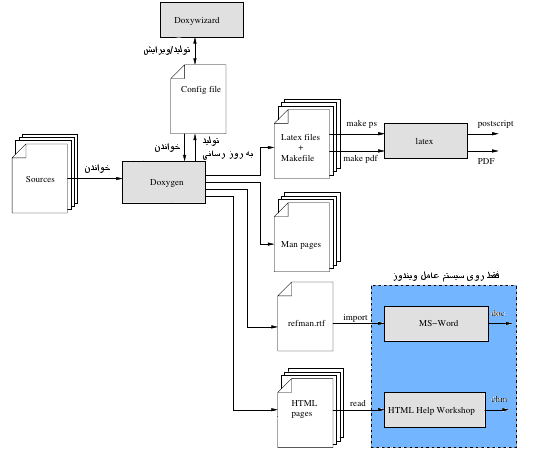
\includegraphics[width=0.75\textwidth]{image/doxygen_doxywizard}
  \caption[ارتباط \lr{Doxygen} و \lr{Doxywizard}.]{
ارتباط \lr{Doxygen} و \lr{Doxywizard}.
\lr{Doxygen} 
برنامه‌ی اصلی برای تولید مستند از پرونده‌های منبع است که برای تولید نیاز به یک پرونده‌ی پیکربندی دارد. \lr{Doxywizard} ساخت 
پرونده‌ی پیکربندی را برای کاربران ساده می‌کند و به کاربران اجازه می‌دهد پرونده‌های پیکربندی را ویرایش کنند. همچنین از طریق آن 
می‌توان \lr{Doxygen} را اجرا کرد.
  }
  \label{doxygen_doxywizard}
\end{figure}

\begin{sloppypar}
\lr{Doxygen} 
 زبان‌های برنامه نویسی بسیاری را حمایت می‌کند. به صورت پیش فرض زبان‌های 
\lr{C}، \lr{C++}، \lr{C\#}، \lr{Objective-C}، \lr{Java}، \lr{PHP}، \lr{Python}، \lr{Fortran}، \lr{IDL}، \lr{VHDL} و \lr{D} 
توسط \lr{Doxygen} حمایت می‌شوند. یعنی اگر پرونده‌هایی که در آن‌ها مستندات و کدهای خود را نوشته‌اید به یکی از این زبان‌ها باشد، 
می توانید با استفاده از \lr{Doxygen}، مستند فنی آن‌ها را تولید کنید. 
البته تجزیه‌کننده\footnote{\lr{Parser}} و پالایه\footnote{\lr{Filter}} برای زبان‌های دیگر نیز توسط افراد یا 
گروه‌های دیگر ساخته شده و یا در حال ساخت است. برای اطلاع از این موارد به آدرس 
\lr{http://www.doxygen.org/helpers.html} 
مراجعه نمایید. \lr{Doxygen} زبان برنامه نویسی نوشته شده در پرونده‌ها را از پسوند پرونده‌ها تشخیص می‌دهد. به عنوان مثال 
اگر پسوند یک پرونده \lr{.f} باشد، \lr{Doxygen} زبان برنامه نویسی نوشته شده در آن پرونده‌را زبان فرترن در نظر می‌گیرد، 
یا اگر پسوند پرونده‌ای \lr{.java} باشد، زبان برنامه نویسی آن پرونده زبان جاوا در نظر گرفته می‌شود. البته می‌توان با 
ویرایش پرونده‌ی پیکربندی، این نوع تشخیص را عوض کرد.
\end{sloppypar}

با استفاده از \lr{Doxygen}  می‌توان مستندات را در قالب‌های مختلفی تولید کرد. قالب‌های 
\lr{HTML}، \lr{LaTeX}، \lr{Man pages}، \lr{RTF}، \lr{XML} و \lr{Qt Help Project (.qhp)} 
در \lr{Doxygen} به صورت مستقیم حمایت می‌شوند، و قالب‌های 
\lr{Qt Compressed Help (.qhc)}، \lr{PostScript (.ps)} و \lr{PDF} 
نیز به طور غیر مستقیم حمایت می‌شوند، به این ترتیب که مستندات در قالب \lr{.qhc} را می‌توان از طریق مستندات 
تولید شده در قالب \lr{.qhp} ساخت و مستندات در قالب \lr{PostScript} و \lr{PDF} را هم می‌توان از طریق مستندات 
تولید شده در قالب \lr{LateX} به دست آورد.


در این فصل، در قسمت اول کار با \lr{Doxygen} از طریق خط فرمان را شرح می‌دهیم و در قسمت بعد، نحوه‌ی استفاده از \lr{Doxywizard} را 
بیان می‌کنیم که یک واسط گرافیکی برای استفاده از \lr{Doxygen} است.
% این قسمت که در واقع قسمتی از بخش استفاده از doxygen و doxywizard است به نحوه
% استفاده از doxygen از طریق خط فرمان می پردازد.
% محمد هادی منصوری ۹۰/۴/۲۵
\section{خط فرمان}

% استفاده از Doxygen به صورت خط فرمان
 همانگونه که در قسمت‌های قبل نیز اشاره شد، \lr{Doxygen} یک برنامه‌ی کاربردی بر
اساس خط فرمان است. اگر در خط فرمان دستور زیر را وارد کنید، که در واقع فراخوانی
\lr{Doxygen} با پارامتر \lr{--help} است، توضیح مختصری از نحوه‌ی استفاده از این
برنامه نمایش داده می شود.

\begin{Shell} 
doxygen --help
\end{Shell}

به طور کلی نحوه‌ی استفاده از این برنامه در خط فرمان به این صورت است: نوشتن
کلمه‌ی \lr{doxygen} و سپس نوشتن پارامترهای لازم برای کاری که می‌خواهیم انجام
دهیم. کلیه‌ی پارامترها به صورت یک یا چند کاراکتر که قبل از آن یک علامت منها (-)
قرار داده می شود، نوشته می‌شوند.

\lr{Doxygen} 
برای تولید مستند نیاز به یک پرونده‌ی پیکربندی دارد. در پرونده‌ی پیکربندی تنظیمات
مربوط به تولید مستندات تعیین می‌گردد. علاوه بر پرونده‌ی پیکربندی باید
پرونده‌هایی که حاوی کدها و مستندات هستند را نیز در اختیار این نرم‌افزار قرار داد
تا برای آن‌ها یک مستند یکپارچه تولید کند.

پس از اینکه مستندات خود را بر اساس قواعدی که در فصل‌های بعدی بیان شده است، 
نوشتید برای تولید مستند با استفاده از \lr{Doxygen} باید مراحل زیر را طی کنید:
\begin{enumerate}
\item ایجاد یک پرونده‌ی پیکربندی اولیه
\item ویرایش پرونده‌ی پیکربندی اولیه در صورت نیاز
\item اجرای نرم‌افزار \lr{Doxygen} و تولید مستند یکپارچه
\end{enumerate}

\subsection{ایجاد پرونده‌ی پیکربندی اولیه}

نوشتن پرونده‌ی پیکربندی به صورت دستی کاری زمانبر است اما برای اینکه ایجاد
پرونده‌ی پیکربندی ساده شود، نرم‌افزار \lr{Doxygen} می‌تواند یک پرونده‌ی پیکربندی
اولیه که حاوی مقادیر پیش‌فرض است، تولید کند. با دستور زیر می‌توان یک پرونده‌ی
پیکربندی اولیه را تولید کرد:

\begin{Shell}  
doxygen -g <config-name>
\end{Shell}

در دستور بالا \lr{<config-name>} نامی است که برای پرونده‌ی تولیدی تعیین می‌شود.
در صورتی که این پارامتر تعیین نشود، یعنی نامی برای پرونده‌ی تولیدی مشخص نشود،
پرونده‌ی تولیدی با نام \lr{Doxyfile} تولید می‌شود.
در صورتی که پرونده‌ای با نام \lr{configName} از قبل وجود داشته باشد،
\lr{Doxygen} ابتدا نام آن پرونده را به \lr{<configName>.bak} تغییر می‌دهد و پس
از آن پرونده‌ی پیکربندی را با نام داده شده تولید می‌کند.
اگر به جای پارامتر \lr{<config-name>} یک علامت منها (\-) قرار داده شود،
\lr{Doxygen} تلاش می‌کند که پرونده‌ی پیکربندی را از ورودی استاندارد \lr{(stdin)}
بخواند.

\subsection{ویرایش پرونده‌ی پیکربندی}

پرونده‌ی پیکربندی قالبی بسیار ساده دارد. این پرونده شامل تعدادی انتساب (تگ) به
یکی از دو صورت زیر است:

\begin{Config}
TAGNAME = VALUE
TAGNAME = VALUE1 VALUE2 ...
\end{Config}

حالت اول برای تنظیماتی است که فقط یک مقدار دارند و صورت دوم برای تنظیماتی است که
می‌توانند چند مقدار داشته باشند.

احتمالاً نیازی به تغییر مقدار اغلب این تگ‌ها ندارید و مقدار پیش‌فرض تعیین شده
برای آن‌ها در پرونده‌ی پیکربندی تولید شده را بدون تغییر خواهید گذاشت.
% برای اطلاعات بیشتر قسمت پیکربندی را مشاهده کنید.

در صورتی که نمی‌خواهید پرونده‌ی پیکربندی را با یک ویرایشگر متن ویرایش کنید،
می‌توانید از نرم‌افزار \lr{Doxywizard} استفاده کنید که یک واسط گرافیکی برای
تولید، خواندن و نوشتن پرونده‌های پیکربندی است و تعیین مقدار تنظیمات مختلف
پیکربندی را از طریق پنجره‌های گرافیکی فراهم می‌سازد. نحوه استفاده از
\lr{doxygen} از طریق واسط گرافیکی \lr{doxywizard} در قسمت‌های بعد شرح داده شده
است.

برای یک پروژه کوچک که شامل تعداد کمی پرونده‌ی منبع (\lr{source}) و سرآیند
(\lr{header}) به زبان \lr{C} و/یا \lr{C++} است، می‌توانید تگ \lr{INPUT} را بدون
مقدار رها کنید. در این حالت \lr{Doxygen} در مسیر جاری به دنبال پرونده‌های منبع
می‌گردد.

اگر پروژه‌ای دارید که شامل یک پوشه از پرونده‌های منبع است و یا شامل چندین پوشه
یا پوشه‌های تو در تو است، باید آدرس پوشه‌ها را در مقابل تگ \lr{INPUT} قرار دهید.
نوع پرونده‌ها یا به عبارتی قالب پرونده‌ها را باید در تگ \lr{FILE\_PATTERNS}
تعیین کنید (مثلا \lr{*.cpp *.h}). تنها پرونده‌هایی که با یکی از الگوهای داده شده
مطابقت داشته باشند توسط \lr{doxygen} تجزیه و تحلیل می‌شوند. در صورتی که در تگ
\lr{FILE\_PATTERNS} الگویی تعیین نشود، \lr{doxygen} فهرستی از پسوندهای مربوط به
پرونده‌های منبع را در نظر می‌گیرد. باید توجه داشت که \lr{doxygen} قالب پرونده‌ها
را از روی پسوند آنها تعیین می‌کند(مثلا \lr{.java} برای پرونده‌های منبع به زبان
جاوا، پسوند \lr{.cpp} برای زبان \lr{C++} و ...). در صورتی که پروژه شامل پوشه‌های
تو در تو است باید آدرس پوشه‌ی ریشه (اصلی) را به تگ \lr{INPUT} منتسب کنید و تگ
\lr{RECURSIVE} را نیز با \lr{YES} مقداردهی کنید. البته راه دیگر این است که آدرس
تمام پوشه‌ها (چه اصلی چه داخلی) را در تگ \lr{INPUT} به طور مستقیم اضافه کنید.

با استفاده از تگ‌های \lr{EXCLUDE} و \lr{EXCLUDE\_PATTERNS} می‌توانید پوشه‌ها یا
پرونده‌هایی را تعیین کنید که نباید تجزیه و تحلیل شوند. فرض کنید درون پوشه یا
پوشه‌هایی که آدرس آن‌ها را در تگ \lr{INPUT} قرار داده‌اید پوشه‌ها یا پرونده‌هایی
وجود دارند که نمی‌خواهید مستند آن‌ها به مستنداتی که توسط \lr{doxygen} تولید
می‌شود اضافه شود. برای این کار از دو تگ یاد شده استفاده می‌شود. در تگ
\lr{EXCLUDE} می‌توان پوشه‌هایی را تعیین کرد که ممکن است درون پوشه‌هایی که در
قسمت \lr{INPUT} تعریف شده‌اند قرار داشته باشند. به این ترتیب در هنگام تجزیه و
تحلیل پرونده‌های منبع، از این پوشه‌ها و پرونده‌های موجود در آن‌ها صرف نظر
می‌شود. با استفاده از تگ \lr{EXCLUDE\_PATTERNS} هم می‌توان الگوهایی را تعیین کرد
تا پرونده‌ها یا پوشه‌هایی که با یکی از این الگوها مطابقت دارند در هنگام تجزیه و
تحلیل در نظر گرفته نشوند. \lr{doxygen} این الگوها را با آدرس مطلق پرونده‌ها و
پوشه‌ها مقایسه می‌کند. به عنوان مثال برای جلوگیری از تجزیه و تحلیل تمام
پرونده‌هایی که در پوشه‌ای با نام \lr{inner} قرار دارند می‌توان به این صورت اقدام
کرد: \lr{EXCLUDE\_PATTERNS = */inner/*}.

\lr{doxygen} 
برای تشخیص اینکه یک پرونده را چگونه تجزیه و تحلیل کند به پسوند پرونده‌ها نگاه
می‌کند. اگر پرونده‌ای دارای پسوند \lr{.idl} یا \lr{.odl} باشد، آن را به عنوان یک
پرونده‌ی \lr{IDL} در نظر می‌گیرد. اگر پرونده‌ای پسوند \lr{.java} داشته باشد آن
را به عنوان یک پرونده که به زبان جاوا نوشته شده است در نظر می‌گیرد. پرونده‌هایی
که انتهای ‌آن‌ها \lr{.cs} است به عنوان پرونده‌های \lr{C\#} و پرونده‌هایی با
پسوند \lr{.py} به عنوان پرونده‌هایی به زبان پایتون \lr{(python)} در نظر گرفته
می‌شوند. در نهایت، پرونده‌هایی که پسوند آن‌ها \lr{.php}، \lr{.php4}، \lr{.inc}
یا \lr{.phtml} است به عنوان پرونده‌های منبع به زبان \lr{PHP} در نظر گرفته
می‌شوند. هر پسوند دیگر باعث می‌شود \lr{doxygen} آن پرونده را به عنوان پرونده‌ای
به زبان \lr{C/C++}، تجزیه و تحلیل کند (البته در صورتی که واقعا به زبان
\lr{C/C++} نوشته شده باشند). پرونده‌هایی که پسوند \lr{.m} دارند به عنوان
\lr{Objective-C} در نظر گرفته می‌شوند.

برای تعیین محلی که مستندات تولید شده توسط \lr{doxygen} باید در آنجا ذخیره شود از
تگ \lr{OUTPUT\_DIRECTORY} استفاده می‌شود. در مقابل این تگ باید نام یا آدرس
پوشه‌ای که مستندات تولیدی باید در آنجا قرار داده شوند نوشته شود.
آدرس داده شده می‌تواند نسبی یا مطلق باشد. آدرس نسبی نسبت به مسیر جاری که
\lr{doxygen} در آن اجرا می‌شود تعیین می‌گردد.
به عنوان مثال اگر در پرونده‌ی پیکربندی تگ \lr{OUTPUT\_DIRECTORY} را به صورت
\lr{OUTPUT\_DIRECTORY = result} مقداردهی کنید، آنگاه \lr{doxygen} در مسیر جاری
به دنبال پوشه‌ای به نام \lr{result} می‌گردد تا مستنداتی را که تولید می‌کند در آن
پوشه ذخیره کند.


اگر  پروژه‌ای دارید که هنوز مستندی که مناسب \lr{doxygen} باشد برای آن ننوشته‌اید
و یا مستندات هنوز کامل نیستند، در این حالت می‌توانید از \lr{doxygen} استفاده
کنید تا ساختار و شکل ظاهری مستندی که تولید می‌شود را مشاهده کنید. برای انجام این
کار باید تگ \lr{EXTRACT\_ALL} را در پرونده‌ی پیکربندی با \lr{YES} مقداردهی کنید.
به این ترتیب \lr{doxygen} مستندی شامل تمام موجودیت‌های پروژه (اعم از کلاس‌ها،
متدها، توابع و ...) تولید می‌کند، حتی اگر برای برخی موجودیت‌ها توضیحی نوشته نشده
باشد. به این نکته باید توجه داشت که موجودیت‌هایی که مستند نشده باشند (یعنی
توضیحی برای آن‌ها نوشته نشده باشد) در مستند تولید شده توسط \lr{doxygen} آورده
نمی‌شوند مگر اینکه تگ \lr{EXTRACT\_ALL} در پرونده‌ی پیکربندی با \lr{YES}
مقداردهی شده باشد. مقدار پیش‌فرض این تگ \lr{NO} است.

برای تحلیل قسمتی از یک نرم‌افزار که از قبل نوشته شده است می‌توان از \lr{doxygen}
کمک گرفت. برای تحلیل یک نرم‌افزار مفید است که برای هر موجودیت، ارجاعاتی به کد
مربوط به آن موجودیت در مستند وجود داشته باشد تا بتوان از طریق آن‌ها به کدهای
مربوطه دسترسی داشت. اگر تگ \lr{SOURCE\_BROWSER} با \lr{YES} مقداردهی شود،
\lr{doxygen} در مستنداتی که تولید می‌کند چنین ارجاعاتی را قرار می‌دهد. همچنین
می‌توان کاری کرد که متن کد مربوط به هر موجودیت به طور مستقیم در مستندات تولید
شده ظاهر شود. برای این کار باید تگ \lr{INLINE\_SOURCES} با \lr{YES} مقداردهی
شود. این کار می‌تواند برای مرور دستی کدهای نوشته شده مفید باشد. به عنوان مثال
فرض کنید می‌خواهید کدهایی را مرور کنید که توسط شخص دیگری نوشته شده است، یا اینکه
بخواهید کدها و مستنداتی که نوشته‌اید را در اختیار برنامه نویس دیگری قرار دهید تا
آن‌ها را مرور کند یا توسعه دهد. تولید اینگونه مستندات در چنین مواردی بسیار مفید
است.

\subsection{اجرای نرم‌افزار \lr{Doxygen} و تولید مستند}

پس از ایجاد و ویرایش پرونده پیکربندی، در این مرحله برای اجرای برنامه
\lr{doxygen} از طریق خط فرمان و تولید مستندات باید از دستور زیر استفاده شود:

\begin{Shell}
doxygen <config-name>
\end{Shell}

در دستور بالا \lr{<config-name>} نام پرونده‌ی پیکربندی است که از قبل تهیه شده است.


بسته به تنظیماتی که در پرونده‌ی پیکربندی قرار داده‌اید، \l{doxygen} یک یا چند
پوشه با نام‌های \lr{html}، \lr{rtf}، \lr{latex}، \lr{xml} و/یا \lr{man} را در
پوشه‌ای که به عنوان پوشه مقصد در تگ \lr{OUTPUT\_DIRECTORY} ذکر کرده‌اید
می‌سازد.این پوشه‌ها همانطور که از نامشان مشخص است حاوی مستندات تولید شده توسط
\lr{doxygen} در قالب‌های \lr{HTML}، \lr{RTF}، \lr{LATEX}، \lr{XML} و/یا
\lr{Unix-Man page} هستند.

مسیر خروجی پیش‌فرض برای ذخیره‌ی مستندات تولید شده، مسیری است که \lr{doxygen} در
آن اجرا شده است.
همانطور که در قسمت قبل گفته شد، مسیر یا پوشه‌ای که خروجی‌ها در آن قرار می‌گیرند
را می‌توان با مقداردهی به تگ \lr{OUTPUT\_DIRECTORY} تغییر داد. نام پوشه‌ی خاص هر
قالب خروجی را هم می‌توان با مقداردهی به تگ‌های \lr{HTML\_OUTPUT}،
\lr{RTF\_OUTPUT}، \lr{LATEX\_OUTPUT}، \lr{XML\_OUTPUT} و/یا \lr{MAN\_OUTPUT} در
پرونده‌ی پیکربندی تغییر داد. در صورتی که پوشه‌ی مربوط به مسیر خروجی تعیین شده
وجود نداشته باشد، \lr{doxygen} سعی می‌کند آن پوشه را بسازد و بعد مستندات تولیدی
را در آن قرار دهد. البته باید توجه داشت که \lr{doxygen} کل پوشه‌های مذکور در
مسیر را نمی‌سازد و فقط داخلی‌ترین پوشه را در صورت عدم وجود می‌سازد. سایر
پوشه‌های پدر در مسیر خروجی باید از قبل وجود داشته باشند.

\subparagraph{خروجی \lr{HTML}}

مستندات تولید شده در قالب \lr{HTML} را می‌توان به وسیله‌ی یک مرورگر \lr{HTML}
باز کرده و مشاهده کرد. صفحه‌ی اصلی (یا صفحه‌ی آغازین) مستندات در این قالب
پرونده‌ی \lr{index.html} در پوشه‌ی \lr{html} است. برای مشاهده‌ی بهترین نتیجه از
این مستندات باید از مرورگری که از \lr{CSS}ها پشتیبانی می کند برای باز کردن و
مشاهده این مستندات استفاده شود (نمایش مستندات تولید شده در قالب \lr{HTML} با
استفاده از مرورگرهای \lr{Mozilla}، \lr{Safari}، \lr{Konqueror}، و \lr{IE6} مناسب
است).

در مستندات \lr{HTML} می‌توان یک فهرست درختی یا نمایی درختی از مطالب موجود در
مستند وارد کرد. برای این کار باید تگ \lr{GENERATE\_TREEVIEW} در پرونده‌ی
پیکربندی با \lr{YES} مقداردهی شود. البته در صورت تولید مستندات با چنین امکانی،
برای مشاهده‌ی آن‌ها نیاز به مرورگرهایی دارید که علاوه بر \lr{CSS}، از \lr{DHTML}
و \lr{JavaScript} نیز حمایت کنند.
تقریباً تمام مرورگرهای جدید از این امکانات حمایت می‌کنند و مشکلی با نمایش
اینگونه مستندات ندارند.


\subparagraph{خروجی \lr{LaTeX}}

مستند \lr{LaTeX} تولید شده توسط \lr{doxygen} ابتدا باید به وسیله‌ی یک مترجم
(کامپایلر) \lr{LaTeX} ترجمه شود. \lr{doxygen} برای ساده سازی روند ترجمه‌ی
مستندات تولید شده یک پرونده‌ی \lr{Makefile} را در پوشه‌ی \lr{LaTeX} قرار می‌دهد.

محتویات پرونده‌ی \lr{Makefile} به مقدار تگ \lr{USE\_PDFLATEX} در پرونده‌ی
پیکربندی بستگی دارد. اگر این تگ غیر فعال شده باشد (یعنی با \lr{NO} مقداردهی شده
باشد)، با اجرای دستور \lr{make} در مسیری که مستندات در
 قالب \lr{LaTeX} تولید شده‌اند، یک پرونده‌ی \lr{dvi} با نام \lr{refman.dvi}
 تولید خواهد شد. این پرونده را می‌توان با
استفاده از \lr{xdvi} مشاهده کرد و یا با اجرای دستور \lr{make ps} به یک پرونده‌ی
\lr{PostScript} تبدیل کرد (این کار نیاز به \lr{dvips} دارد). این پرونده را
می‌توان به \lr{PDF} هم تبدیل کرد، البته در صورتی که مفسر \lr{ghostscript} نصب
شده باشد. برای تبدیل به \lr{PDF} کافی است دستور \lr{make pdf} را اجرا کنید.

برای اینکه خروجی \lr{PDF} بهتری داشته باشید باید تگ‌های \lr{PDF\_HYPERLINK} و
\lr{USE\_PDFLATEX} در پرونده پیکربندی را با \lr{YES} مقداردهی کنید. در این صورت
پرونده‌ی \lr{Makefile} موجود در پوشه‌ی مستندات \lr{LaTex}، تنها حاوی دستوراتی
برای ایجاد \lr{refman.pdf} خواهد بود.

\subparagraph{خروجی \lr{RTF}}

\lr{Doxygen} 
برای تولید مستندات در قالب \lr{RTF} تنها یک پرونده به نام \lr{refman.rtf} تولید
می‌کند و تمام مستندات را در همان یک پرونده قرار می‌دهد. این پرونده برای وارد
کردن (\lr{import}) در مایکروسافت وورد (\lr{Microsoft Word}) بهینه شده است.
برخی اطلاعات با استفاده از \lr{field} کدگذاری شده‌اند. برای نمایش مقدار واقعی
باید تمام آن‌ها را انتخاب کنید (یعنی گزینه‌ی \lr{Edit-> Select all} را بزنید) و
سپس \lr{fielf} را عوض کنید (با کلیک راست و انتخاب گزینه‌ی \lr{option} از منویی
که ظاهر می‌شود).

\subparagraph{ خروجی \lr{XML} }

خروجی \lr{XML} تولیدی توسط \lr{doxygen} شامل مجموعه‌ای ساختار یافته از اطلاعاتی
است که به وسیله‌ی \lr{doxygen} جمع‌آوری می‌شود.
هر مولفه (کلاس، فضای نام، پرونده و ...) پرونده‌ی \lr{xml} مربوط به خود را دارد.
علاوه بر آن‌ها یک پرونده‌ی شاخص به نام \lr{index.xml} نیز وجود دارد.
 
یک پرونده به نام \lr{combine.xslt} نیز تولید می‌شود که می‌تواند برای ترکیب تمام
پرونده‌های \lr{xml} در یک پرونده به کار رود.

\subparagraph{خروجی \lr{Man page}}

در مورد مستندات تولیدی در قالب \lr{Man-page} باید به این نکته توجه داشت که این
قالب محدودیت‌های محدودی دارد. بنابراین برخی اطلاعات (مثل دیاگرام کلاس‌ها،
ارجاعات و فرمول‌ها) از دست خواهند رفت.

%
% حق نشر 1390-1402 دانش پژوهان ققنوس
% حقوق این اثر محفوظ است.
% 
% استفاده مجدد از متن و یا نتایج این اثر در هر شکل غیر قانونی است مگر اینکه متن حق
% نشر بالا در ابتدای تمامی مستندهای و یا برنامه‌های به دست آمده از این اثر
% بازنویسی شود. این کار باید برای تمامی مستندها، متنهای تبلیغاتی برنامه‌های
% کاربردی و سایر مواردی که از این اثر به دست می‌آید مندرج شده و در قسمت تقدیر از
% صاحب این اثر نام برده شود.
% 
% نام گروه دانش پژوهان ققنوس ممکن است در محصولات دست آمده شده از این اثر درج
% نشود که در این حالت با مطالبی که در بالا اورده شده در تضاد نیست. برای اطلاع
% بیشتر در مورد حق نشر آدرس زیر مراجعه کنید:
% 
% http://dpq.co.ir/licence
%
%استفاده از {\lr{Doxygen}} به صورت گرافیکی (با استفاده از {\lr{Doxywizard}})
\section{گرافیکی (با استفاده از \lr{Doxywizard})}

\lr{Doxywizard} 
یک برنامه گرافیکی برای پیکربندی و اجرای \lr{doxygen} است. با اجرای این برنامه یک
پنجره اصلی (که بسته به سیستم عاملی که دارید ظاهر آن متفاوت است) نمایش داده
می‌شود(برای نمونه تصویر \ref{پنجره_داکسی_ویزارد} را ببینید).
با استفاده از امکانات گرافیکی موجود در این برنامه می‌توان \lr{doxygen} را
پیکربندی و اجرا کرد. به طور کلی با استفاده از \lr{doxywizard} می توان کارهای زیر
را انجام داد:

\begin{itemize}
 \item
پیکربندی \lr{doxygen} و ذخیره آن به صورت یک پرونده متنی برای استفاده‌های بعدی.
\item
باز کردن و ویرایش یک پرونده پیکربندی که از قبل تهیه شده.
\item
اجرای \lr{doxygen} برای تولید مستندات بر اساس پیکربندی تعیین شده.
\end{itemize}

\begin{figure}
\centering
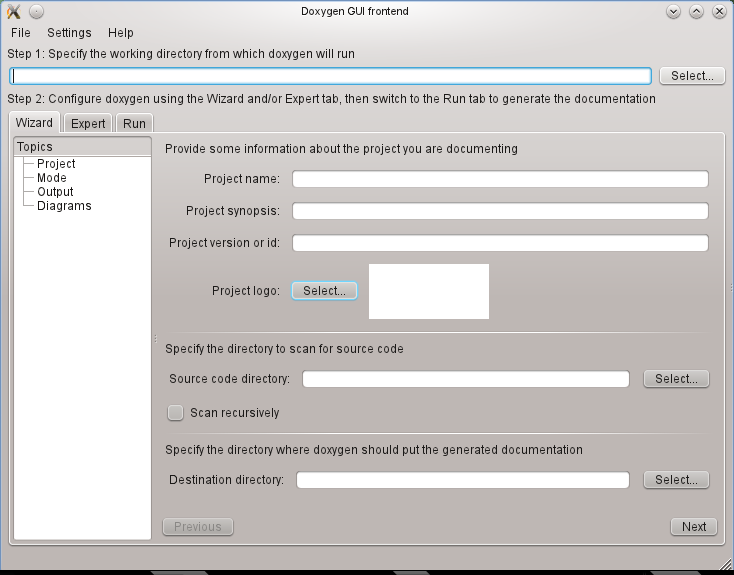
\includegraphics[width=0.75\textwidth]{image/doxywizard_linux}
\caption[نمونه‌ای از پنجره اصلی برنامه گرافیکی \lr{Doxywizard}.]
{
نمونه‌ای از پنجره اصلی برنامه گرافیکی \lr{Doxywizard}. با استفاده از امکانات گرافیکی موجود در این برنامه می‌توان پرونده‌های پیکربندی را تهیه و ویرایش کرد و برنامه \lr{Doxygen} را نیز به اجرا درآورد.
}
\label{پنجره_داکسی_ویزارد}
\end{figure}


همانطور که قبلاً هم گفته شد، برای تولید مستندات از کدهای منبع با استفاده از
\lr{dowygen} ابتدا باید یک پرونده پیکربندی تهیه کرد تا \lr{doxygen} بر اساس آن
اقدام به تولید مستندات کند. در ادامه توضیح داده می‌شود که چگونه می‌توان با
استفاده از امکانات گرافیکی موجود در \lr{doxywizard} یک پرونده پیکربندی تهیه کرد
و \lr{doxygen} را اجرا کرد.

\subsection{پیکربندی}

برای پیکربندی \lr{doxygen} از طریق \lr{doxywizard} سه روش وجود دارد که در ادامه
این روش‌ها را شرح می‌دهیم.

\paragraph{روش اول: استفاده از پرونده پیکربندی از قبل موجود.}
در صورتی که یک پرونده پیکربندی آماده دارید و اکنون می‌خواهید همان پیکربندی را به
کار ببرید و یا اینکه می‌خواهید آن را کمی ویرایش کنید و سپس از آن استفاده کنید،
می‌توانید از منوی \lr{File} گزینه \lr{Open} را انتخاب کنید (البته در برخی موارد
دکمه‌ای تحت عنوان \lr{Load} برای این کار است وجود دارد). با این کار
\lr{doxywizard} پرونده مربوطه را خوانده و تنظیمات درج شده در آن را در قسمت‌های
مختلف نمایش می‌دهد. در صورت نیاز می‌توانید هر قسمت را که می‌خواهید ویرایش کنید.

\paragraph{روش دوم: پیکربندی سریع.}
در صورتی که بخواهید فقط تنظیمات مهم را تعیین کنید و سایر جزئیات و تنظیمات را با
مقدار پیش‌فرض رها کنید تب \lr{Wizard} را انتخاب کنید. با انتخاب این تب در فهرست
سمت چپ چهار آیتم \lr{Project}، \lr{Mode}، \lr{Output} و \lr{Diagram} را مشاهده
خواهید کرد. این چهار آیتم در واقع چهار مرحله برای تنظیمات است. در هر مرحله
تنظیمات خاصی تعیین می‌شود. در زیر این مراحل شرح داده شده است:

\subparagraph{\lr{Project}}
در این قسمت تنظیمات عمومی مربوط به پروژه‌ای که مستندات آن تولید خواهد شد تعیین
می‌شود. این تنظیمات عبارتند از:
نام پروژه، خلاصه‌ای از پروژه، شماره نسخه پروژه، لوگوی پروژه و آدرس پوشه‌ای که
پرونده‌های منبع (کدها و توضیحات) پروژه در آن قرار دارد. علاوه بر آن‌ها گزینه‌ای
تحت عنوان \lr{Scan recursively} وجود دارد. این گزینه برای مواقعی است که درون
پوشه حاوی کدهای منبع، پوشه‌های دیگری نیز وجود داشته باشد که پرونده‌های درون این
پوشه‌ها هم باید در تولید مستند استفاده شوند (به عبارتی پروژه حاوی پوشه‌های تو در
تو باشد). آخرین آیتم این مرحله تعیین آدرس پوشه‌ای است که مستندات تولید شده توسط
\lr{doxygen} باید در آن قرار گیرند (یعنی آدرس پوشه نتایج).

در بالاترین قسمت پنجره \lr{doxywizard} محلی وجود دارد که در آن می‌توان پوشه‌ یا
آدرسی را که \lr{doxygen} باید در آن اجرا شود، تعیین کرد. اگر آدرس پوشه
پرونده‌های منبع یا پوشه نتایج زیر پوشه‌ای از آدرس داده شده باشند، می‌توان آدرس
آن‌ها را به صورت نسبی، نسبت به پوشه مذکور وارد کرد. در غیر این صورت باید حتما
آدرس‌ها به صورت مطلق داده شوند.

\subparagraph{\lr{Mode}}
در این قسمت نحوه استخراج مستندات از کدها منبع تعیین می‌شود. در بخش اول تعیین
می‌شود که آیا کلیه موجودیت‌ها (کلاس‌ها، متدها، توابع و \ldots) در مستند تولیدی
آورده شوند (\lr{All Entities}) یا اینکه فقط موجودیت‌هایی که مستند شده‌اند در
مستند ظاهر شوند (\lr{Docuented entities only}).

در صورتی که بخواهید ارجاعات یا پیوندهایی به اصل کدها در مستندات وجود داشته باشد
باید گزینه \lr{Include cross-referenced \ldots} تیک زده شود (این کار در واقع
معادل با مقداردهی تگ \lr{SOURCE\_BROWSING} با مقدار \lr{YES} در پرونده پیکربندی
است).

در بخش دوم این تب می‌توان زبان برنامه‌نویسی پروژه را تعیین کرد تا مستندات تولیدی
برای زبان مربوطه بهینه شود.

\subparagraph{\lr{Output}}
این قسمت تنظیمات مربوط به خروجی‌های \lr{doxygen} است. در این قسمت می‌توان تعیین
کرد که مستندات در چه قالبی تولید شوند. قالب‌های ممکن عبارتند از: \lr{HTML}،
\lr{\LaTeX}، \lr{Man page}، \lr{RTF} و \lr{XML}.
برای دو قالب \lr{HTML} و \lr{\LaTeX} تنظیمات بیشتری نیز وجود دارد.

در قسمت \lr{HTML} می‌توان تعیین کرد که مستندات تولید شده در قالب \lr{HTML} فقط
حاوی \lr{HTML} ساده باشد، حاوی بخش دسترسی سریع\footnote{\lr{Navigation panel}}
باشد یا اینکه در قالب \lr{.chm} باشد. همچنین می‌توان تعیین کرد که قسمت جستجو در
صفحات \lr{html} وجود داشته باشد یا نه. برای این کار باید گزینه \lr{With search
function} را علامت‌دار یا بدون علامت کرد.

در تنظیمات مربوط به قالب \lr{HTML} دکمه‌ای تحت عنوان \lr{Change color \ldots}
وجود دارد که با استفاده از آن می‌توان رنگ عمومی صفحات \lr{HTML} را تعیین کرد. با
فشردن این دکمه پنجره‌ای نمایش داده می‌شود که در سمت راست آن سه نوار رنگی قرار
دارد. با تغییر فلش مربوط به این نوارهای رنگی می‌توانید رنگ مورد نظر خود را تعیین
کنید.


در قسمت \lr{LaTeX} می‌توان تعیین کرد که مستندات در قالب \lr{\LaTeX} به عنوان یک
قالب میانی برای تولید \lr{PDF} است یا \lr{PostScript}.

به این نکته توجه داشته باشید که در هر صورت \lr{Doxygen} پرونده‌های مربوط به
کدهای منبع را تغییر نمی‌دهد و فقط آن‌ها را می‌خواند.

\subparagraph{\lr{Diagram}}
\lr{Doxygen} 
می‌تواند دیاگرام‌هایی را در مستندات تولید کند. در این قسمت تعیین می‌شود که چه
دیاگرام‌هایی و چگونه تولید شوند.
بیشتر دیاگرام‌ها به ابزار \lr{dot} از بسته \lr{GraphViz}\footnote{ برای کسب
اطلاعات بیشتر درباره این بسته نرم‌افزاری و دریافت آن می‌توانید به آدرس
\lr{http://www.graphviz.org} مراجعه نمایید.} نیاز دارند. در حالت کلی سه گزینه
برای انتخاب وجود دارد: مستندات بدون دیاگرام تولید شوند، از تولید کننده داخلی
برای تولید کلاس دیاگرام استفاده شود، یا اینکه از ابزار \lr{dot} از بسته
\lr{GraphViz} برای تولید دیاگرام استفاده شود.

\paragraph{روش سوم: پیکربندی با جزئیات کامل.}
برای دسترسی به کلیه تنظیمات ممکن در پرونده پیکربندی و ویرایش تنظیمات مورد نظر
می‌توان از تب \lr{Expert} استفاده کرد. در این قسمت تمام تنظیماتی که در یک پرونده
پیکربندی \lr{doxygen} وجود دارد قابل مشاهده است. برای نظم بیشتر و دسترسی راحت‌تر
این تنظیمات در در ۱۶ گروه دسته‌بندی شده‌اند. نام گروه‌ها در فهرست سمت چپ در تب
\lr{Expert} مشاهده می‌شود.
البته به این نکته توجه داشته باشید که می‌توانید تنظیمات مورد نظر خود را از
قسمت‌های مختلف (هم از قسمت \lr{Wizard} و هم از قسمت \lr{Expert}) تعیین کنید.

اگر محتویات یک پرونده پیکربندی را مشاهده کنید می‌بینید که تنظیمات مختلف به نوعی
دسته‌بندی شده‌اند. گروه‌های مختلفی که در فهرست سمت چپ از تب \lr{Expert} مشاهده
می‌کنید در واقع همان دسته‌بندی را نشان می‌دهند که در اینجا نمایی گرافیکی دارد.
در هر گروه از تب \lr{Expert}، برای هر مورد قابل تنظیم (به عبارتی برای هر تگ) در
پرونده پیکربندی یک عنصر گرافیکی تهیه شده است. عنصر گرافیکی مربوط به هر تگ، به
نوع آن تگ و  مقدار یا مقادیری که می‌تواند بگیرد بستگی دارد.

% مطالب مربوط به صفحه ۸۴ از مستند کاربری داکسی ژن
\begin{itemize}
 \item 
برای تنظیماتی که از نوع بولی (تنظیماتی که در پرونده پیکربندی با مقادیر \lr{YES} یا \lr{NO} مقداردهی می‌شوند دکمه‌ای 
برای علامت زدن (یا \lr{check-box}) وجود دارد.
\item
برای تنظیماتی که می‌توانند مقادیر خاص و معین بگیرند (مثل تگ \lr{OUTPUT\_LANGUAGE} که زبان مستندات تولید شده را 
تعیین می‌کند) یک فهرست انتخاب (یا \lr{combo box} در نظر گرفته شده است.
\item
برای تنظیماتی که مقادیر عددی از بازه‌ای خاص را می‌توانند بگیرند یک \lr{spinbox} در نظر گرفته شده است.
\item
برای تنظیماتی که می‌توانند یک رشته (یا یک جمله) را به عنوان مقدار دریافت کنند، یک جعبه ویرایش تک 
خطی (\lr{one line edit field}) در نظر گرفته شده است.
\item
برای تنظیماتی که می‌توانند چند رشته (یا چند کلمه) را به عنوان مقدار دریافت کنند (مثل تگ \lr{FILE\_PATTERNS}) یک 
جعبه ویرایش تک خطی به همراه سه دکمه '+'، '-' و '*' و یک فهرست در نظر گرفته شده است. با نوشتن یک رشته در جعبه 
ویرایش و زدن دکمه '+' رشته مورد نظر به فهرست اضافه می‌شود. با انتخاب یک رشته از فهرست و زدن دکمه '-' آن رشته 
حذف می‌شود. با انتخاب یک رشته از فهرست و تغییر آن و سپس زدن دکمه '*' تغییرات داده شده در رشته انتخاب شده در فهرست 
اعمال می‌شود (به عبارتی رشته جدید با رشته قبلی جایگزین می‌شود).
\item
برای تنظیماتی که یک پرونده یا یک پوشه را به عنوان مقدار دریافت می‌کنند دکمه‌ای وجود دارد که با فشردن آن، پنجره‌ای 
برای انتخاب پرونده یا پوشه ظاهر می‌شود.
\end{itemize}

برای مشاهده توضیحات مربوط به هر آیتم یا معنی آن، کافی است اشاره‌گر ماوس را روی
آیتم مورد نظر ببرید. در این حالت در پنجره‌ای که در قسمت پایین سمت چپ قرار دارد
توضیحاتی در مورد آیتم نمایش داده می‌شود (در برخی موارد در قسمت پایین سمت راست
دکمه‌ای تحت عنوان راهنما (\lr{Help}) قرار دارد که با زدن این دکمه و سپس کلیک روی
آیتم مورد نظر، توضیحات مربوط به آن آیتم به نمایش درمی‌آید).

\subsection{اجرای \lr{Doxygen}}

برای اجرای \lr{doxygen} از طریق \lr{doxywizard} باید تب \lr{Run} را انتخاب کنید.
در این تب می‌توانید تنظیماتی که تعیین کرده‌اید را ببینید. برای مشاهده دکمه
\lr{Show configuration} را بزنید. با این کار کلیه تنظیمات (هم آن‌هایی که ویرایش
کرده‌اید، هم آن‌ها که به صورت پیش‌فرض رها کرده‌اید) مشاهده می‌شود که از طریق
دکمه \lr{Save log} می‌توانید آن‌ها را در به صورت یک پرونده متنی ذخیره کنید تا در
صورت نیاز بعداً به صورت دستی و یا از طریق همین برنامه \lr{doxywizard} آن را باز
کرده و ویرایش کنید.

با زدن دکمه \lr{Run doxygen} یا \lr{Start} برنامه \lr{doxygen} با توجه به
تنظیماتی که تعیین کرده‌اید شروع به کار می‌کند و در حین تولید مستندات، گزارشی از
کارهایی که در حال انجام است نیز نمایش داده می‌شود. این گزارش‌ها را نیز می‌توان
از طریق همان دکمه \lr{Save log} به عنوان یک پرونده متنی ذخیره کرد. هنگام اجرای
\lr{doxygen} اگر از ادامه کار منصرف شدید می‌توانید با زدن همان دکمه قبلی از
ادامه کار \lr{doxygen} جلوگیری کنید.

پس از اتمام تولید مستندات توسط \lr{doxygen}، می‌توان از طریق دکمه \lr{Show HTML
output} به صفحه اول مستندات تولیدی در قالب \lr{HTML} رجوع کرد. البته در صورتی که
در پیکربندی اولیه، تولید مستندات در قالب \lr{HTML} را فعال نکرده باشید این دکمه
غیرفعال خواهد بود زیرا \lr{doxygen} مستندی در قالب \lr{HTML} تولید نکرده است.
